\section{Approximate $k$-List in Euclidean norm} \label{sec:Approx_kList_Euclid}

The problem we are going solve in this section is the following special case of the $k$-List problem. This problem is at the heart of sieving algorithms for the Shortest Vector Problem.


\begin{definition}[Approximate $k$-List problem in $l_2$-norm] \label{def:kListL2}
Let $0 < t < \sqrt{k}$. Given $k$ lists $L_1, \ldots, L_k$ of equal exponential size whose elements are iid.\ uniformly chosen vectors from the $n$-sphere $\Sphere{n}$, the task is to output a $1-\smallo(1)$-fraction of $k$-tuples $\xvec_1 \in L_1, \ldots, \xvec_k \in L_k$ s.t.\ $\|\xvec_1 + \ldots + \xvec_k \|^2 \leq t^2$. Such a tuple $(\xvec_1, \ldots, \xvec_k)$ is called a solution to the approximate $k$-List problem. 
\end{definition}

We analyze the case where $t$ and $k$ are constant and the input lists are of size $2^{\const n}$ for some constant $\const$. The restriction $t < \sqrt{k}$ is set to get a meaningful problem. Due to the fact that for large $n$, random vectors $\xvec_i$'s from $\Sphere{n}$ are almost orthogonal with high probability (cf.\ Thm.~\ref{thm:WishartDist}), a $1-\smallo(1)$-fraction of tuples $(\xvec_1, \ldots, \xvec_k) \in L_1 \times \ldots \times L_k$ satisfy $\| \xvec_1 + \ldots + \xvec_k \|^2 \approx k$. So the problem is non-trivial when either $t< \sqrt{k}$, or $t>\sqrt{k}$. We concentrate on the former. With a simple modification our results apply to the latter case as well. Moreover, our algorithm works for lists of different sizes, but it would unnecessarily complicate the analysis, so we stick to lists of equal size. Additionally, equally-sized lists is a relevant scenario for the \SVP-sieving algorithms.

In the applications to sieving (see Sect.~\ref{subsec:ApproxSVP}), we have $t=1$ and look for solutions with the property $\|\xvec_1 \pm \ldots \pm \xvec_2 \| \leq 1$. Since there are $2^k  = \bigO(1)$ possible choices for signs, we can consider each choice separately increasing the running time of the algorithm by a constant factor. %It leads to few optimizations considered in Sect.~\ref{subsec:KListResults}, but they do not change the asymptotics.

\subsection{Configurations} \label{subsec:ConfigL2}

All the $k$-List algorithms make use of the fact that there are many solution-tuples and we are allowed to output a fraction of all the solutions. 
The main challenge in designing an efficient $k$-List algorithm is to identify a criterion s.t.\ (1) a solution that matches the criterion is easy to find, and (2) enough solutions satisfy this criterion.  The first property leads to a faster algorithm, the second is specified by the problem. In the case of the approximate $k$-List problem, we want to output almost all solutions.

To define the criterion we use in our algorithm, recall the definition of a Gram matrix.

\begin{definition}[Gram Matrix]
 For vectors $\xvec_1, \ldots, \xvec_k$ from $\R^n$, the \emph{Gram matrix} $C \in \R^{k \times k}$ is a positive semidefinite matrix whose entries are pairwise inner products: $C_{i, j} = \ScProd{x_i}{x_j}$.
\end{definition}  

Note that the Gram matrix is invariant under simultaneous rotations and reflections of all $\xvec_i$'s. This property also holds for a $k$-tuple from $\Sphere{n}$ that forms a solution to the approximate $k$-List problem as both, rotation and reflection, preserve distance. Hence, we are interested in solutions up to such symmetry. We set our searching criteria to be a specific Gram matrix of vectors $\xvec_1, \ldots, \xvec_k$ which we call a \emph{configuration}. 

\begin{definition}[Configuration] \label{def:Configuration}
	The \emph{configuration} $C = \Conf(\xvec_1, \ldots, \xvec_k)$ for $\xvec_1, \ldots, \xvec_k \in \Sphere{n}$ is the Gram matrix $C_{i, j} = \ScProd{x_i}{x_j}$.
\end{definition}

The configuration gives all the necessary information on the geometry of the tuple, and in particular
\begin{equation} \label{eq:LengthOfSum}
 \| \sum_i \xvec_i \|^2 = \sum_i \| \xvec_i \|^2 + \sum_{i \neq j} \ScProd{\xvec_i}{\xvec_j} = k + 2 \sum_{i<j}\ScProd{\xvec_i}{\xvec_j}.
\end{equation}

Let us define the space of all possible configurations for $\xvec_i \in \Sphere{n}$ together with the space of those configurations that give a tuple with the property $\| \sum_i \xvec_i \|^2 \leq t$:
\begin{align*}
	&\ConfSpace = \{ C \in \R^{k \times k} \; |  \; C \text{ symmetric positive semi-definite}, C_{i,i}=1 \}, \\
	&\ConfSpacet = \{ C \in \ConfSpace \; | \; \sum_{i,j} C_{i,j} \leq t^2 \}.
\end{align*}

For fixed $k$, we think of the set $\ConfSpace$ as a finite set which we can efficiently enumerate.  
Observing that a tuple $(\xvec_1, \ldots, \xvec_k)$ is a solution to the approximate $k$-List problem iff $\Conf(\xvec_1, \ldots, \xvec_k) \in \ConfSpacet$, immediately gives us an algorithm: we enumerate over all configurations in $\ConfSpacet$ and solve the \emph{$k$-List configuration problem} defined as follows.

\begin{definition}[Configuration Problem] \label{def:ConfigProblem}
Given $k$ exponentially sized lists $L_1, \ldots, L_k$ of vectors from $\Sphere{n}$, a target configuration $C \in \ConfSpace$, and $\eps>0$, the task is to output \emph{all} $k$-tuples $\xvec_1 \in L_1, \ldots, \xvec_k \in L_k$ s.t.\ $| \ScProd{\xvec_i}{\xvec_j} - C_{i,j}| \leq \eps$ for all $i, j$. Such a tuple is called a solution to the Configuration problem.
\end{definition}

\begin{remark}
To simplify the analysis, we assume we can compute with real numbers. Our algorithm and the analysis remain true when we use sufficiently precise approximations. Since the inner products $\ScProd{\xvec_i}{\xvec_j}$ take real values, asking for the exact equality to $C$ does not bring any solution. We, therefore, introduce some small $\eps > 0$. For two configurations $C, C'$, we write $C \approx_{\eps} C'$ when $| C_{i,j} - C'_{i,j} | \leq \eps$. 
\end{remark}

The crucial property of a solution $(\xvec_1, \ldots, \xvec_k)$ to the Configuration problem is the fact that it can be \emph{locally} verified as we only have to look at \emph{pairs} $\xvec_i, \xvec_j$. Note that a solution to the approximate $k$-List problem as given in Def.~\ref{def:kListL2} does not share this `locality' feature. 

Now we have an algorithm to solve the $k$-List problem: (1) enumerate all the configurations $C \in \ConfSpacet$, and (2) solve the Configuration problem for each $C$. Below we show how to bypass the first step. It turns out that we do not have to enumerate all the configurations to output a $1-\smallo(1)$-fraction of the solutions to the $k$-List problem. There exist one particular configuration, later denoted as $\Cbalt$, which is attained by most of the solutions. This allows us to solve the Configuration problem only for $\Cbalt$ to obtain enough solution-tuples for the $k$-List problem. To give $\Cbalt$ explicitly, we study the Wishart distribution \cite{Wishart28}, which is a matrix generalization of the chi-squared distribution.

\paragraph{Wishart distribution.} Consider $k$ vectors $\xvec_1, \ldots, \xvec_k \in \R^{n+1}$ sampled independently from $(n+1)-$ dimensional spherical Gaussian (mean $0$ and standard deviation\ $1$). Set $S_{i,j} = \ScProd{\xvec_i}{\xvec_j} \in \R^{k \times k}$. For integer $k, n$ with $n+1 > k-1$, a random $k \times k$ symmetric matrix $S$ has a Wishart distribution with the probability density function
\begin{equation} \label{eq:WishartDensity}
	\pW(S) = \frac{e^{-\tfrac{1}{2} \cdot \Tr S} \cdot \det(S)^{\frac{n-k}{2}}}{2^{\frac{(n+1)k}{2}} \pi^{\frac{k (k-1)}{4}} \prod_{i=0}^{k-1} \Gamma \bigl( \frac{n+1-i}{2} \bigr)}  \d S,
\end{equation}
where $\d S = \prod_{i \leq j} \d S_{i,j}$, $\Gamma(z) = \int\limits_0^\infty x^{z-1} e^{-x}\d x$ is the Gamma-function, and $\Tr(S)$ is the trace-function (i.e., the sum of the main-diagonal elements of $S$). A derivation of these density can be found in \cite{Eaton07}. 

Note that matrix $S$ is a Gram matrix of vectors \emph{not} from $\Sphere{n}$. To get the density function for distribution on our configuration space $\ConfSpace$ where vectors are sampled uniformly from the $n$-sphere, we have to normalize $S$ and change the reference density $\d S$ appropriately. 

\begin{thm} \label{thm:WishartDist}
Let $\xvec_1, \ldots, \xvec_k \in \Sphere{n}$ be independent uniformly distributed on the $n$-sphere, $n > k$. Then the configuration $C = \Conf(\xvec_1, \ldots, \xvec_k)$ follows a distribution $\pC$ on $\ConfSpace$ with the probability density function
\[
	\pC (C) = W_{n,k} \cdot \det(C)^{\tfrac{1}{2}(n-k)} \d \ConfSpace = \softO_k \Bigl( \det(C)^{\tfrac{n}{2}}\Bigr) \d \ConfSpace,
\]
where $\d \ConfSpace = \d C_{1,2} \cdots \d C_{k-1, k}$ and $W_{n,k} = \pi^{-\frac{k(k-1)}{4}} \prod_{i=0}^{k-1} \frac{\Gamma \bigl( \frac{n+1}{2} \bigr)}{\Gamma\bigl( \frac{n+1-i}{2} \bigr)} = \softO_k\Bigl( n^{\frac{(k-1)k}{4}} \Bigr)$ is a normalization constant that only depends on $n$ and $k$.
\end{thm}

\begin{proof}
	Let $C_{i,j} = \frac{S_{i,j}}{\sqrt{S_{i,i} S_{j,j}}}$, where $S$ follows the Wishart distribution with pdf given in Eq.~(\ref{eq:WishartDensity}). This normalization defines the map $\Phi$ from $\R^{\frac{k(k+1)}{2}}$ to itself that represents the following change of variables:
	\begin{align*}
		\Phi&(S_{1,1}, S_{2,2}, \ldots, S_{k,k}, S_{1,2}, \ldots, S_{1,k}, S_{2,3}, \ldots, S_{k-1, k}) = \\
		&(S_{1,1}, S_{2,2}, \ldots, S_{k,k}, \tfrac{S_{1,2}}{\sqrt{S_{1,1} S_{2,2}}}, \ldots, \tfrac{S_{1,k}}{\sqrt{S_{1,1} S_{k,k}}}, \tfrac{S_{2,3}}{\sqrt{S_{2,2} S_{3,3}}}, \ldots, \tfrac{S_{k-1,k}}{\sqrt{S_{k-1,k-1} S_{k,k}}}) = \\
		&(S_{1,1}, S_{2,2}, \ldots, S_{k,k}, C_{1,2}, \ldots, C_{1, k}, C_{2,3}, \ldots, C_{k-1, k}).
	\end{align*}
	Note that we keep the diagonal elements $S_{i,i}$ to make the transformation $\Phi$ injective, as we want to apply the substitution rule $\prod_{i=1}^k \d S_{i,i} \prod_{i <j} C_{i,j} = | \det (D \Phi) | \cdot \prod_{i \leq j} \d A_{i,j}$, where $D \Phi$ is the Jacobian of $\Phi$. This Jacobian is a triangular matrix with the main diagonal 
	\[(1, \ldots, 1, \frac{1}{\sqrt{S_{1,1} S_{2,2}}}, \ldots, \frac{1}{\sqrt{S_{1,1} S_{k,k}}}, \frac{1}{\sqrt{S_{2,2} S_{3,3}}}, \ldots, \frac{1}{\sqrt{S_{k-1,k-1} S_{k,k}}}),  
	\]
	so its determinant is $|\det (D \Phi)|  = \prod_i \frac{1}{\sqrt{S_{i,i}}^{k-1}}$.
	Further, we can express $S$ as $S = T C T$, where $T$ is a diagonal matrix with $(\sqrt{S_{1,1}}, \ldots, \sqrt{S_{k,k}})$ on the main diagonal. Therefore, $\det(S) = \det(C) \cdot \prod_i S_{i,i}$. Applying the transformation to the Wishart density function, one readily obtains a pdf.\ in $(S_{1,1}, \ldots, S_{k,k}, C_{1,2}, \ldots, C_{k-1,k})$-variables
	\begin{equation} \label{eq:rhoWishProof}
		\pW = \frac{ e^{-\frac12\sum_i S_{i,i}} \det(C)^{\frac{n-k}{2}} \prod_i S_{i,i}^{\frac{n-k}{2}}}{2^{\frac{(n+1)k}{2}} \pi^{\frac{k(k-1)}{4}} \prod_{i=0}^{k-1} \Gamma(\frac{n-i+1}{2} ) } \prod_i\sqrt{S_{i,i}}^{k-1}\prod_i \d S_{i,i}\prod_{i<j}\d C_{i,j}.
	\end{equation}
	As we want to relate the distribution to $C_{i,j}$ only, we integrate over $\prod_i \d S_{i,i}$ to obtain the desired $\pC$. From Eq.~(\ref{eq:rhoWishProof}), it follows that $\pC$ is of the form $\pW = W_{n,k} \det(C)^{\frac{n-k}{2}} \d \ConfSpace$ for some factor $W_{n,k}$ that depends only on $k$ and $n$. We write $W_{n,k}$ as $W_{n,k} = \frac{1}{t} e^{-\frac12\sum_i S_{i,i}} \prod_i S_{i,i}^{\frac{n-k}{2}}$, where $t$ is the denominator in Eq.~(\ref{eq:rhoWishProof}), and compute
	\begin{align*}
		W_{n,k} &= \frac{1}{t} \idotsint\limits_{A_{1,1}\hspace{1.3em}A_{k,k}} e^{-\frac12\sum_i S_{i,i}} \prod_i S_{i,i}^{\frac{n-k}{2}} \prod_i\sqrt{S_{i,i}}^{k-1}\prod_i \d S_{i,i} \\
		&=\frac{1}{t} \idotsint\limits_{A_{1,1}\hspace{1.3em}A_{k,k}}e^{-\frac12\sum_i S_{i,i}} \prod_i S_{i,i}^{\frac{n-1}{2}}\prod_i \d S_{i,i} \\
		&=\frac{1}{t} \Bigl( \int\limits_{S_{1,1}=0}^{+ \infty} S_{1,1}^{\frac{n-1}{2}} e^{-\frac12 S_{1,1}} \d S_{1,1}\Bigr)^k \\
		&=\frac{2^{\frac{k(n+1)}{2}}}{t} \Bigl( \int\limits_{S_{1,1}=0}^{+ \infty} \Bigl( \frac{S_{1,1}}{2} \Bigr)^{\frac{n+1}{2} - 1} e^{-\frac12 S_{1,1}} \d \frac{S_{1,1}}{2}\Bigr)^k \\
		&=\frac{2^{\frac{k(n+1)}{2}}}{t} \Bigl( \int\limits_{x=0}^{+ \infty} x^{\frac{n+1}{2}-1} e^{-x} \d x \Bigr)^k \\
		&=\frac{2^{\frac{k(n+1)}{2}} \cdot \Gamma \Bigl( \frac{n+1}{2} \Bigr)^k}{t}
		=\frac{\Gamma \bigl( \frac{n+1}{2} \bigr)^k}{\pi^{\frac{k(k-1)}{4}} \prod_{i=0}^{k-1} \Gamma(\frac{n-i+1}{2} )}.
	\end{align*}
	From Stirling's formula, $\Gamma(n) \sim \bigl( \tfrac{n}{e} \bigr)^n$, we have for any fixed $z$ and $n \rightarrow \infty$, $\frac{\Gamma(n+z)}{\Gamma(n)} = \bigO_z(n^z)$. Finally, we have
	\[
		W_{n,k} = \bigO_k \Bigl( n^{\sum_{i=0}^{k-1} \tfrac{i}{2}}\Bigr) = \bigO_k \Bigl( n^{\frac{k(k-1)}{4}} \Bigr).
	\]
\end{proof}

Since we now know the distribution on the space $\ConfSpace$, we want to find a configuration $C \in \ConfSpace$ with the largest mass. It turns out that this is a configuration with the highest amount of symmetry, i.e.\ when all off-diagonal entries are equal. We prove this statement in Thm.~\ref{thm:maxConfig} below. We call such configurations \emph{balanced} and denote them $\Cbal$.

\begin{definition}[Balanced Configuration] \label{def:BalancedConfig}
 A configuration $\Cbal \in \ConfSpace$ is balanced if $C_{i,j} = C_{i', j'}$ for all $i \neq i', j \neq j'$. A balanced configuration that additionally belongs to $\ConfSpacet$ for some target length $t>0$ is denoted $\Cbalt$.
\end{definition} 

Before showing that $\pC$ indeed attains its maximum at $\Cbal$, we compute the determinant of $\Cbal$.
\begin{lemma} \label{lem:CBalancedDet}
\text{Let }
\begin{align*}
C = \begin{psmallmatrix}
         1 & a & a &\ldots & a\\
         a & 1 & a &\ldots & a\\
         a & a & 1 &\ldots & a\\
         & \vdots& &\ddots & \vdots\\
         a & a & a &\ldots & 1
         \end{psmallmatrix}\in\R^{k\times k}.
\end{align*}
Then $\det(C) = (1-a)^{k-1}(1+(k-1)a)$.
\end{lemma}
\begin{proof}
	We write $C = (1-a) \cdot \Id_k + a \cdot \onevec \cdot \onevec^t$. Sylvester's Determinant Identity states that $\det(\Id_m + AB) = \det(\Id_n + BA)$ for any $A$ and $B$ of dimensions $m \times n$ resp.\ $n \times m$. It follows that
	\begin{align*}
	\det(C) &=  \det \bigl( (1-a) (\Id_k + \tfrac{a}{a-1} \onevec \cdot \onevec^t) \bigr) = (1-a)^k \det \bigl( \Id_1 + \tfrac{a}{a-1} \onevec^t \cdot \onevec \bigr) \\
	&=(1-a)^k \bigl( 1 + \tfrac{a}{1-a}k \bigr) = (1-a)^{k-1} (1+(k-1)a).
	\end{align*}  
\end{proof}

The space of all configurations $\ConfSpace$ is compact\footnote{Closeness immediately follows from the fact that $\ConfSpace \subset \R^{k^2}$; further, all entries of an element from $\ConfSpace$ are bounded, in particular, $C_{i,j}\leq 1$.} and, therefore, integrating over it will asymptotically pick the maximum value. So the probability that a uniform random tuple $(\xvec_1, \ldots, \xvec_k)$ forms a  ``good'' configuration from $\ConfSpacet$, and consequently, gives a solution to the Configuration problem, is
\[
 \int\limits_{\ConfSpacet} \pC = \softO(\max\limits_{C \in \ConfSpacet} \det(C)^{n/2}).
\]

The next theorem determines this maximum.

\begin{thm} \label{thm:maxConfig}
	Let $0 < t < \sqrt{k}$ be a target length and $\ConfSpacet \subset \ConfSpace$ be the subset of configurations with target length at most $t$. Then $\det(C)$ attains its unique maximum over $\ConfSpacet$ at the balanced configuration $\Cbalt$ with $C_{i,j} = \frac{t^2-k}{k^2-k}$ for all $i \neq j$ with maximal value
	\[
		\det(\Cbalt) = \frac{t^2}{k} \left( \frac{k^2-t^2}{k^2-k} \right)^{k-1}.
	\] 
	In particular, for $t=1$, $C_{i,j} = -\frac{1}{k}$ and $\det(\CbalOne) = \frac{(k+1)^{k-1}}{k^k}$.
\end{thm}

\begin{proof}
	For $k=2$, the statement immediately follows from Eq.~(\ref{eq:LengthOfSum}). So assume $k \geq 3$. 
	
	Consider configurations $C$ with $\Tr(C) = k$ and $\sum_{i,j} C_{i,j} \leq t^2$. This is clearly weaker than the condition $C_{i,i}=1$ and later we show that the stronger condition is met at the maximum.
	
	From the fact that $C$ is a Gram matrix, and hence, it is positive semi-definite, it follows that its eigenvectors $\vvec_1, \ldots, \vvec_k$ form an orthonormal basis and its eigenvalues $0 \leq \lambda_1 \leq \ldots \leq \lambda_k$ are positive. 
	
	We have $\Tr(C) = \sum_i \lambda_i$ and $\det(C) = \prod_i(\lambda_i)$. We want to find $\lambda_i$'s that maximize the determinant. In particular, we show that $\onevec$ is an eigenvector for maximal $\det(C)$. To see this, write $\sum_{i,j} C_{i,j}  = \onevec C \onevec\transpose$, so for the smallest eigenvalue $\lambda_1$ it holds
	\begin{equation} \label{eq:SmallestEigenvalue}
		t^2 \geq \onevec C \onevec\transpose \geq \lambda_1 \| \onevec \|^2 = k \lambda_1.
	\end{equation}
	We have $\lambda_1 \leq \tfrac{t^2}{k} < 1$. The Arithmetic Mean-Geometric Mean inequality stating that for non-negative real $x_i$'s, $ \tfrac{\sum_i x_i}{n} \geq \sqrt[n]{\prod_i x_i}$, gives for $\det(C) = \lambda_1 \prod_{i=2}^k \lambda_i$ and $\sum_{i=2}^k \lambda_i = k - \lambda_1$:
	\[
			\det(C) \leq \lambda_1 \left( \frac{k-\lambda_1}{k-1} \right)^{k-1}.
	\]
	As the derivative of the right-hand side w.r.t.\ $\lambda_1$, $ \tfrac{k(1-\lambda_1)}{k-1} \bigl( \tfrac{k-\lambda_1}{k-1} \bigr) ^{k-2} > 0$, is everywhere positive, we bound $\det(C)$ by plugging in the maximal $\lambda_1 = \tfrac{t^2}{k}$:
	\begin{equation} \label{eq:IneqForDetC}
		\det(C) \leq \lambda_1 \left( \frac{k-\lambda_1}{k-1} \right)^{k-1} \leq \frac{t^2}{k} \left( \frac{k - \tfrac{t^2}{k}}{k-1}\right)^{k-1} = \frac{t^2}{k} \left( \frac{k^2 - t^2}{k^2-k}\right)^{k-1}.
	\end{equation}
	The first inequality in Eq.~(\ref{eq:IneqForDetC}) becomes an equality iff $\lambda_2 = \ldots = \lambda_k$ and the second  when $\lambda_1  = \tfrac{t^2}{k}$. In this case, from $\Tr(C) = k$, we have $\lambda_2 = \tfrac{k^2-t^2}{k(k-1)}$ and $\onevec$ is an eigenvector of $C$ with eigenvalue $\lambda_1$. 
	
	Now we show that $C_{i,i} = 1$ for maximal $\det(C)$ and $C_{i,j}$ for $i \neq j$ as in the theorem statement. Consider the eigendecomposition $C = V \Lambda V^{-1} = V \Lambda V\transpose$, where $V$ is the orthonormal matrix with $\vvec_i$'s as columns, $\Lambda$ is the diagonal matrix with $\lambda_i$'s on the main diagonal. Equivalently, we can write
	\[
		C = \sum_i \lambda_i \vvec_i \vvec\transpose_i  = (\lambda_1 - \lambda_2) \vvec_1 \vvec\transpose_1 + \lambda_2 \sum\limits_{i=1}^k \vvec_i \vvec\transpose_i = \frac{\lambda_1 - \lambda_2}{k} \onevec \onevec\transpose + \lambda_2 \Id_k.
	\]
	Therefore, all the diagonal entries of $C$ are equal to $\tfrac{\lambda_1 - \lambda_2}{k} + \lambda_2$ and all the off-diagonal entries are equal to $\frac{\lambda_1 - \lambda_2}{k}$. The theorem follows once we substitute the eigenvalues $\lambda_1 = \tfrac{t^2}{k}$, $\lambda_2 = \tfrac{k^2 - t^2}{k(k-1)}$ for maximal $\det(C)$.
\end{proof}

In case we search for configurations with the target length $t > \sqrt{k}$, the proof should consider the largest eigenvalue $\lambda_k$ instead of the smallest $\lambda_1$.

Also from the above proof it follows that looking at `only-1' linear combination of $\xvec_i$'s is optimal. If instead we look for $\| \sum_i a_i \xvec_i \| \leq t$ for some $\avec \neq \onevec$, the set of `good' configurations $\ConfSpacet$ would be $\{ C \in \ConfSpace \; | \; \| \avec\transpose C \avec \| \leq t  \}$ and in the proof above the eigenvector $\onevec$ would be replaced by $\avec$. Since $\onevec$ has the minimal norm, the configurations from $\ConfSpacet$ we are looking at are optimal.

In case $t=1$, the balanced configuration $(\xvec_1, \ldots, \xvec_k)$ forms a regular $k+1$-dimensional simplex with center in the origin (the condition on pair-wise inner products $\ScProd{\xvec_i}{\xvec_j} = -\tfrac{1}{k}$ matches with the central angle for the regular simplex). The missing $k+1\st$ point of the simplex is $-\sum_i \xvec_i$, i.e.\ the negative of the sum (see Fig.~\ref{fig:Tetrahedron}).

From our concentration result, it follows that a random $k$-tuple from $\Sphere{n}$ is a solution to the Configuration problem with probability $\softO( \det(\Cbalt)^{n/2})$. Since we know the size of input list $L_i$, we can compute the expected number of solutions.

\begin{figure}[t]
	\centering
	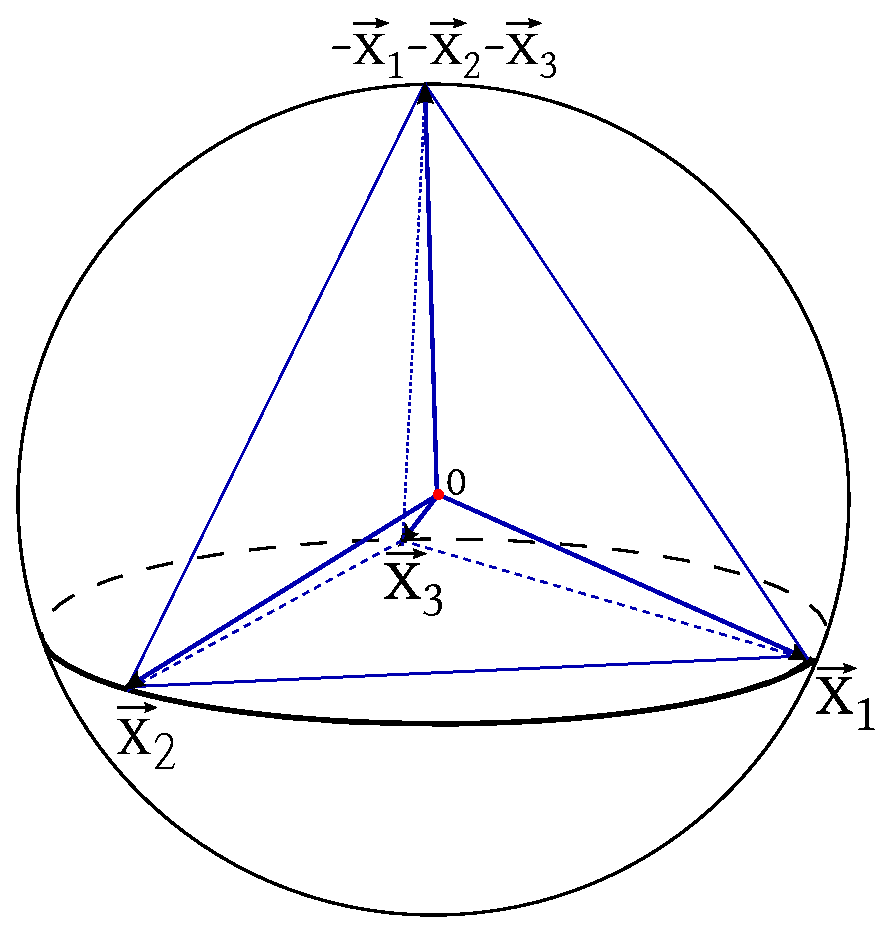
\includegraphics[scale=0.38]{tetrahedron}
	\caption[Balanced Configuration]{A regular tetrahedron ($3-$simplex) represents a balanced configuration for $k=3$.}
	\label{fig:Tetrahedron}
\end{figure}

\begin{corollary} \label{cor:NumberOfSolutions}
	Let $k,t$ be fixed. Then the expected number of solutions to the Configuration problem with input lists of size $|L|$ is
	\begin{equation} \label{eq:ExpNumberOfSolutions}
	\E[\# \text{solutions}] = \softO \left( |L|^k \Bigl(\frac{t^2}{k} \Bigl( \frac{k^2-t^2}{k^2-k} \Bigr)^{k-1}  \Bigr)^{\tfrac{n}{2}} \right).
	\end{equation}
\end{corollary}
\begin{proof}
	The total number of $k$-tuples is $|L|^k$. From Thms.~\ref{thm:WishartDist} and \ref{thm:maxConfig}, the probability that a random $k$-tuple forms a configuration from $\ConfSpacet$ is $\softO( \det(\Cbalt)^{n/2})$. Thm.~\ref{thm:maxConfig} states the value for this determinant.
\end{proof}

As a consequence, we can easily compute the size of input lists for a desired output list's size. In algorithms for \SVP, $t=1$ and the output list is required to have the same size as input lists. The following corollary proves the conjecture stated in \cite{BLS16}.

\begin{corollary} \label{cor:BalancedListSizes}
Let $k$ be fixed and $t=1$. In the Configuration problem, for the input lists each of size $|L|$, the output list is expected to be of size $|L|$ if $|L|  = \softO \Bigl( \Bigl( \frac{k^{\tfrac{k}{k-1}}}{k+1} \Bigr)^{\tfrac{n}{2}} \Bigr)$. 
\end{corollary}
\begin{proof}
	The statement immediately follows from setting the expression in Eq.~(\ref{eq:ExpNumberOfSolutions}) equal to $|L|$ for $t=1$. 
\end{proof}

Finally, we argue that solving the Configuration Problem gives a $1-\smallo(1)$ fraction of solutions for the $k$-List problem. This follows from Thm.~\ref{thm:maxConfig}. Essentially it states that for any fixed $\eps>0$, the probability that a randomly chosen solution to the approximate $k$-List problem forms a configuration $\eps$-close to $\Cbalt$, converges exponentially to $1$ as $n \rightarrow \infty$. Therefore, solving the $k$-List Configuration problem for $\CbalOne$ and restricting to only those solutions whose sum is at most $t$, gives a $1-\smallo(1)$ fraction of solutions for the approximate $k$-List problem. These arguments justify the following corollary.

\begin{corollary}\label{cor:ReductionToConfigProblem}
Let $k,t$ be fixed. Then the approximate $k$-List problem with target length $t$ can be solved in the same time as the $k$-List configuration problem with target configuration $\Cbalt$ for any fixed $\eps>0$.
\end{corollary}

\subsection{Algorithm} \label{subsec:KListAlgL2}

\begin{algorithm}[H]
\caption{$k$-List for the Configuration Problem}
\label{alg:AlgConfig}
\textbf{Input:} $L_1, \ldots, L_k$ -- lists of vectors from $\Sphere{n}$. $\Conf_{i,j}=\ScProd{\xvec_i}{\xvec_j} \in \R^{k \times k}$ -- Gram matrix. $\eps>0$. \\
\textbf{Output:} $\Lout$ -- list of $k$-tuples $\xvec_1 \in L_1, \ldots, \xvec_k \in L_k$, s.t.\ $\abs{\ScProd{\xvec_i}{\xvec_j}-\Conf_{ij}} \leq \eps$, for all $i,j$.

\begin{algorithmic}[1]

\State $\Lout \gets \{ \}$ 
\ForAll { $\xvec_1 \in L_1$}
	\ForAll {$j=2 \ldots k$}
		\State $L_j^{(1)} \gets$ \Call{Filter}{$\xvec_1, L_j, \Conf_{1,j}, \eps$} 
	\EndFor
	
	\ForAll {$\xvec_2 \in L_2^{(1)}$}
		\ForAll {$j=3 \ldots k$}
			\State $L_j^{(2)} \gets$ \Call{Filter}{$\xvec_2, L_j^{(1)}, \Conf_{2,j}, \eps$} 
		\EndFor	
		\State $\ddots$
		\Indent
			\ForAll {$\xvec_k \in L_k^{(k-1)}$}
				\State $\Lout \gets \Lout  \union \{(\xvec_1, \ldots \xvec_k)\}$
			\EndFor
		\EndIndent
	\EndFor
\EndFor 

\State{} \Return{$\Lout$} 
\end{algorithmic}
\vspace{10pt}
\begin{algorithmic}[1]
	\Function{Filter}{$\xvec, L, c, \eps$}
		\State $L' \gets \{ \}$
		\ForAll {$\xvec' \in L$}	
			\If{$\abs{\ScProd{\xvec}{\xvec'} - c}  \leq \eps$}
			 	\State $L' \gets L' \cup \{ \xvec' \}$
			\EndIf	
		\EndFor
		\State{} \Return $L'$
	\EndFunction
\end{algorithmic}

\end{algorithm}

Now we are ready to describe our algorithm for the Configuration problem given in Def.~\ref{def:ConfigProblem}.

On input the algorithm receives $k$ lists $L_1, \ldots, L_k$, a target configuration $\Conf$ in the form of a Gram matrix $\Conf_{i,j}=\langle{\xvec_i,}{\xvec_j}\rangle \in \R^{k \times k}$ and a small $\eps>0$.
The algorithm proceeds as follows: it picks an $\xvec_1 \in L_1$ and filters all the remaining lists with respect to the values $\ScProd{\xvec_1}{\xvec_i}$ for all $2 \leq i \leq k$.
More precisely, $\xvec_i \in L_i$ `survives' the filter if $\abs{\ScProd{\xvec_1}{\xvec_i} - \Conf_{1,i}}  \leq \eps$.
We put such an $\xvec_i$ into $L_i^{(1)}$ (the superscript indicates how many filters were applied to the original list $L_i$).
On this step, all the $k$-tuples of the form $(\xvec_1, \xvec_2, \ldots, \xvec_k) \in \{\xvec_1\} \times L_2^{(1)} \times \ldots \times L_k^{(1)}$ with the first vector $\xvec_1$ fixed partially match the target configuration. 
Most importantly, the lists $L_i^{(1)}$ become much shorter than the original ones. 

Next, we take $\xvec_2 \in L_2^{(1)}$ and create smaller lists $L_i^{(2)}$ from $L_i^{(1)}$ by filtering out all the $\xvec_i \in L_i^{(1)}$ that do not satisfy $\abs{\ScProd{\xvec_2}{\xvec_i} - \Conf_{2,i}}  \leq \eps$ for all $3 \leq i \leq k$.
A tuple of the form $(\xvec_1, \xvec_2, \xvec_3, \ldots, \xvec_k) \in \{\xvec_1\} \times \{\xvec_2\} \times L_3^{(2)} \times \ldots \times  L_k^{(2)}$ satisfies the target configuration $\Conf_{i,j}$ for $i=1,2$. Now we have the first two vectors fixed. 

We proceed with this list-filtering strategy until we have all $\xvec_i$ for $1\le i \le k$ fixed.
We output all the survived $k$-tuples.
Note that our algorithm becomes the trivial brute-force search algorithm once we are down to 2 lists $L_{k-1}^{(k-2)}, L_k^{(k-2)}$.
As soon as we have fixed $\xvec_1,\ldots,\xvec_{k-2}$ and created $L_{k-1}^{(k-2)},L_{k}^{(k-2)}$, we iterate over $L_{k-1}^{(k-2)}$ and check scalar products with every element from $L_{k}^{(k-2)}$. Our algorithm is detailed in Alg.~\ref{alg:AlgConfig}.

In Fig.~\ref{fig:AlgDescription}, we stress the difference between our algorithm (left) and the algorithm for the Configuration problem presented in \cite{BLS16} (right). While not being stated in terms of configurations, the BLS algorithm actually does search for tuples that form the balanced configuration but differently: for a fixed $\xvec_1$, it only filters the next list $L_2$ and the remaining $L_3, \ldots, L_k$ are left unchanged. Once $\xvec_2 \in L_2^{(1)}$ is chosen next, $L_3^{(2)}$ is obtained by applying filtering to the input $L_3$, while our Alg.~\ref{alg:AlgConfig} filters a smaller $L_3^{(1)}$. Certainly, in our approach we can miss some solutions that would be found by the BLS algorithm, but the results of Sect.~\ref{subsec:ConfigL2} show that this is a tiny fraction of solutions which vanishes in the asymptotics. To see the effect of this fact in practice, we refer the reader to Sect.~\ref{subsec:KListResults}.
\clearpage

\begin{figure}
\centering
\begin{subfigure}[t]{0.45\textwidth}
	\begin{tikzpicture}
	\tikzset{
    List/.style={
    rectangle, 
    rounded corners, 
    draw=black, thick,
    minimum width=0.9cm, 
    text centered},
    Vertex/.style={
  	ellipse,
  	draw=black, thick,
  	inner sep=1pt},
	}
	\matrix (m) [row sep=2mm, column sep=2.3mm, name=m] {
		\node[List, minimum height=50pt] (L1) {$L_1$}; &
	 	\node[List, minimum height=50pt] (L2) {$L_2$}; &
		\node[List, minimum height=50pt] (L3) {$L_3$}; &	 	
	 	\node[] {$\ldots$}; &
	 	\node[List, minimum height=50pt] (Lk) {$L_k$}; \\
	 	
	 	\node[Vertex, label=below:{\footnotesize $\xvec_1$}] (x1) {}; &
	 	\node[Vertex] (l12) {\tiny Filter}; &
	 	\node[Vertex] (l13) {\tiny Filter}; &
	 	\node[] (dots1) {}; &
	 	\node[Vertex] (l1k) {\tiny Filter}; \\
	 	
	 	\node[] {}; &
	 	\node[List, minimum height=35pt] (L2p) {$L_2^{(1)}$}; &
		\node[List, minimum height=35pt] (L3p) {$L_3^{(1)}$}; &	 	
	 	\node[] {$\ldots$}; &
	 	\node[List, minimum height=35pt] (Lkp) {$L_k^{(1)}$}; \\
	 	
	 	\node[] {}; &
	 	\node[Vertex, label=below:{\footnotesize $\xvec_2$}] (x2) {}; &
	 	\node[Vertex] (l23) {\tiny Filter}; &
	 	\node[] (dots2) {}; &
	 	\node[Vertex] (l2k) {\tiny Filter}; \\
	 	
	 	\node[] {}; &
	 	\node[] {}; &
	 	\node[List, minimum height=20pt] (L3pp) {$L_3^{(2)}$}; &
	 	\node[] {}; &
	 	\node[List, minimum height=20pt] (Lkpp) {$L_k^{(2)}$}; \\
	 	
	 	\node[] {}; &
	 	\node[] {}; &
	 	\node[] {}; &
	 	\node[] {}; &
	 	\node[] {$\vdots$};\\
	 	
	 	\node[] {}; &
	 	\node[] {}; &
	 	\node[] {}; &
	 	\node[List, minimum height=17pt] (Llast1) {\small $L_{\scalebox{0.5}{ $k-1$}}^{\scriptscriptstyle(k-2)}$}; &
	 	\node[List, minimum height=17pt] (Llast2) {\small $L_{\scalebox{0.5}{$k$}}^{\scriptscriptstyle(k-2)}$};\\
	 	
	 	\node[minimum height=10pt] {}; &
	 	\node[] {}; &
	 	\node[] {}; &
	 	\node[] {}; &
	 	\node[] {}; & \\
	 	
	 	\node[minimum height=10pt] {}; &
	 	\node[] {}; &
	 	\node[] {}; &
	 	\multicolumn{2}{r}{\node[List, minimum height=17pt] (Lout) {\small $\Lout$};} \\
	 };
	%\node[fit=(m-9-3)(m-9-5)] (Lout) {\small $\Lout$};
	 \draw (L1) -- (x1);
	 \draw[->] (x1) -- (l12);
	 \draw[->] (L2) -- (l12);
	 \draw[->] (l12) -- (L2p);
	 
	 \draw (l12) -- (l13);
	 \draw[->](L3) -- (l13);
	 \draw[->] (l13) -- (L3p);
	 
	 \draw[->] (dots1) -- (l1k);
	 \draw[->] (Lk) -- (l1k);
	 \draw[->] (l1k) -- (Lkp);
	 
	 \draw (L2p) -- (x2);
	 \draw[->] (x2) -- (l23);
	 \draw[->] (L3p) -- (l23);
	 \draw[->] (l23) -- (L3pp);
	 
	 \draw[->] (dots2) -- (l2k);
	 \draw[->] (Lkp) -- (l2k);
	 \draw[->] (l2k) -- (Lkpp);
	 
	 \draw[->] (Llast1) -- (44pt, -112pt);
	 \draw[->] (Llast2) -- (45pt, -112pt);	
	 
\end{tikzpicture}
\caption{\footnotesize Pictorial representation of Alg.~\ref{alg:AlgConfig}. At level $i$, a filter receives as input $\xvec_i \in L_i^{(i-1)}$ and a vector $\xvec_{j}$ from $L_{j}^{(i-1)}$ (for the input lists, $L = L^{(0)}$). $\xvec_j$ passes through the filter if $\abs{\ScProd{\xvec_i}{\xvec_j} - \Conf_{i,j}}  \leq \eps$, in which case it is added to $L_{j}^{(i)}$. All the vectors from $L_j^{(i-1)}$ for all $j \leq i+1$ are processed in this manner. The configuration $\Conf$ and $\eps>0$ are global parameters.}
\label{fig:AlgDescription}
\end{subfigure} %
\quad \quad
\begin{subfigure}[t]{0.47\textwidth}
	\begin{tikzpicture}
	\tikzset{
    List/.style={
    rectangle, 
    rounded corners, 
    draw=black, thick,
    minimum width=0.9cm, 
    text centered},
    Vertex/.style={
  	ellipse,
  	draw=black, thick,
  	inner sep=1pt},
	}
	\matrix (m) [row sep=1.6mm, column sep=2.3mm] {
		\node[List, minimum height=50pt] (L1) {$L_1$}; &
	 	\node[List, minimum height=50pt] (L2) {$L_2$}; &
		\node[List, minimum height=50pt] (L3) {$L_3$}; &	 	
	 	\node[] {$\ldots$}; &
	 	\node[List, minimum height=50pt] (Lk) {$L_k$}; \\
	 	
	 	\node[Vertex, label=below:{\footnotesize $\xvec_1$}] (x1) {}; &
	 	\node[Vertex] (l12) {\tiny Filter}; &
	 	\node[] (l13) {}; &
	 	\node[] (dots1) {}; &
	 	\node[] (l1k) {}; \\
	 	
	 	\node[] {}; &
	 	\node[List, minimum height=35pt] (L2p) {$L_2^{(1)}$}; &
		\node[] (L3p) {}; &	 	
	 	\node[] {$\ldots$}; &
	 	\node[] (Lkp) {}; \\
	 	
	 	\node[] {}; &
	 	\node[Vertex, label=below:{\footnotesize $\xvec_2$}] (x2) {}; &
	 	\node[Vertex] (l23) {\tiny Filter}; &
	 	\node[] (dots2) {}; &
	 	\node[] (l2k) {$\vdots$}; \\
	 	
	 	\node[] {}; &
	 	\node[] {}; &
	 	\node[List, minimum height=20pt] (L3pp) {$L_3^{(2)}$}; &
	 	\node[] {$\vdots$}; &
	 	\node[] (Lkpp) {}; \\
	 	
	 	\node[] {}; &
	 	\node[] {}; &
	 	\node[] {}; &
	 	\node[] {}; &
	 	\node[] {}; & \\[-1.3ex]
	 	
	 	\node[] {}; &
	 	\node[] {}; &
	 	\node[] {}; &
	 	\node[List, minimum height=17pt] (Llast1) {\small $L_{\scalebox{0.5}{ $k-1$}}^{\scriptscriptstyle(k-2)}$}; &
	 	\node[] {};\\
	 	
	 	\node[] {}; &
	 	\node[] {}; &
	 	\node[] {}; &
	 	\node[] {}; &
	 	\node[List, minimum height=17pt] (Llast2) {\small $L_{\scalebox{0.5}{ $k$}}^{\scriptscriptstyle(k-2)}$}; \\
	 	
	 	\node[minimum height=10pt] {}; &
	 	\node[] {}; &
	 	\node[] {}; &
	 	\node[] {}; &
	 	\node[] {}; & \\
	 	
	 	\node[minimum height=10pt] {}; &
	 	\node[] {}; &
	 	\node[] {}; &
	 	\multicolumn{2}{r}{\node[List, minimum height=17pt] (Lout) {\small $\Lout$};} \\
	 };
	 \draw (L1) -- (x1);
	 \draw[->] (x1) -- (l12);
	 \draw[->] (L2) -- (l12);
	 \draw[->] (l12) -- (L2p);
	 
	 %\draw (l12) -- (l13);
	 \draw[->](L3) -- (l23);
	 \draw[->] (l23) -- (L3pp);
	 
	 %\draw[->] (dots1) -- (l1k);
	 %\draw[->] (Lk) -- (l1k);
	 %\draw[->] (l1k) -- (Lkp);
	 
	 \draw (L2p) -- (x2);
	 \draw[->] (x2) -- (l23);
	 %\draw[->] (L3p) -- (l23);
	 %\draw[->] (l23) -- (L3pp);
	 
	 %\draw[->] (dots2) -- (l2k);
	 \draw[-] (Lk) -- (l2k);
	 \draw[->] (l2k) -- (Llast2);
	 \draw[->] (Llast1) -- (44pt, -112pt);
	 \draw[->] (Llast2) -- (45pt, -112pt);	
\end{tikzpicture}
\caption{\footnotesize The $k$-List algorithm given in \cite{BLS16}. The main difference is that a filter receives as inputs $\xvec_i$ and a vector $\xvec_j \in L_j$, as opposed to $\xvec_j \in L_j^{(i-1)}$. Technically, in \cite{BLS16}, $\xvec_i$ survives the filter if $\normalabs{\ScProd{\xvec_i}{\xvec_1+\ldots+\xvec_{i-1}}} \geq c_i$ for some predefined $c_i$. Due to our concentration results, this description is equivalent to the one given in \cite{BLS16} in the sense that the returned solutions are (up to a sub-exponential fraction) the same.}
\label{fig:AlgBLS}
\end{subfigure}
\caption[$k$-List algorithms for the Configuration problem]{$k$-List Algorithms for the Configuration Problem (Def.~\ref{def:ConfigProblem}). Left: Our Alg.~\ref{alg:AlgConfig}. Right: The algorithm from \cite{BLS16}}
\end{figure}

\clearpage

\subsection{Analysis} \label{subsec:KListAnalysisL2}

In this section we analyze the complexity of Alg.~\ref{alg:AlgConfig} for the Configuration problem. First, we should mention that the memory complexity is completely determined by the input list-sizes $\abs{L_i}$ (remember that we restrict to constant $k$) and the application of $k$ filters does not change the asymtotics. In practice, all intermediate lists $L_i^{(j)}$ can be implemented by storing pointers to the elements of the original lists. 

In the following, we compute the expected sizes of filtered lists $L_i^{(j)}$ and establish the expected running time of Alg.~\ref{alg:AlgConfig}. Since our algorithm has an exponential running time $2^{cn}$ for some $c = \Theta(1)$, we are interested in determining $c$. We ignore polynomial factors, e.g.\ we do not take into account time spent for computing inner products. 

\begin{thm}\label{thm:RunTimeAlg1}
Let $k$ be fixed. Alg.~\ref{alg:AlgConfig} given as input $k$ lists $L_1, \ldots, L_k \subset \Sphere{n}$ of the same size $\abs{L}$, a target balanced configuration $\Cbalt \in \R^{k \times k}$, a target length $0 < t < \sqrt{k}$, and $\eps > 0$, outputs the list $\Lout$ of solutions to the Configuration problem. The expected running time of Alg.~\ref{alg:AlgConfig} is
	\begin{equation}\label{eq:RunTime}
	 T =  \softO \Bigl( \abs{L} \cdot \max\limits_{1 \leq i \leq k-1}  \abs{L}^i \cdot \frac{(k^2-t^2)^i}{(k^2-k)^{i+1}}  \cdot \Bigl( \frac{(k^2 - k + (i-1)(t^2-k))^2}{k^2 - k +(i-2)(t^2-k)} \Bigr)^{\frac{n}{2}} \Bigr).
  \end{equation}
In particular, for $t=1$ and $\abs{\Lout} = \abs{L}$ it holds that
  \begin{equation}\label{eq:RunTime=1}
	 T = \softO \biggl( \Bigl( \frac{k^{ \frac{1}{k-1} }}{k+1} \cdot  \max\limits_{1 \leq i \leq k-1} k^{\frac{i}{k-1}} \cdot \frac{(k-i+1)^2}{k-i+2}  \Bigr)^{\frac{n}{2}} \biggr).
  \end{equation}
\end{thm}

\begin{remark}\label{rmk:RunningTimeOfBLS} In the proof below we also show that the expected running time of 
the BLS
$k$-List algorithm 
from \cite{BLS16} for $t=1,\abs{\Lout}=\abs{L}$ is
\begin{equation} \label{eq:RunTimeBLS}
	T_{\text{BLS}} = \softO \Bigl(  \Bigl( \frac{k^{\frac{k}{k-1}}}{(k+1)^2} \cdot \max\limits_{1 \leq i \leq k-1} \bigl( k^{\frac{i}{k-1}} \cdot (k-i+1) \bigr)\Bigr)^{\frac{n}{2}} \Bigr).
\end{equation}
\end{remark} 

\begin{proof}[Proof of Thm.~\ref{thm:RunTimeAlg1}]
	The correctness of the algorithm is straightforward: let us associate the lists $L^{(i)}$ with a level $i$, where $i$ indicates the number of filtering steps applied to $L$ (we identify the input lists with the $0\th$ level: $L_i=L^{(0)}_i$). So for executing the filtering for the $i\th$ time, we choose an $\xvec_{i} \in L_{i}^{(i-1)}$ that satisfies the condition $\abs{\ScProd{\xvec_i}{\xvec_{i-1}} - C_{i,i-1}} \leq \eps$ (for a fixed $\xvec_{i-1}$) and append to a previously obtained $(i-1)$-tuple $(\xvec_1, \ldots, \xvec_{i-1})$. Thus, on the last level, we put into $\Lout$ a $k$-tuple $(\xvec_1, \ldots, \xvec_{k})$ that is a solution to the Configuration problem. To make the subscripts less confusing, we set $C = \Cbalt$ throughout the proof. 
	
	Let us first estimate the size of the list $L_i^{(i-1)}$ output by the filtering process applied to the list $L_i^{(i-2)}$ for $i>1$ (i.e.\ the left-most lists in Fig.~\ref{fig:AlgDescription}). Recall that all $\xvec_i \in L_i^{(i-1)}$ satisfy $\abs{\ScProd{\xvec_i}{\xvec_{j}} - C_{i,j}} \leq \eps$, $1 \leq j \leq i-1 $. Then the \emph{total} number of $i$-tuples $(\xvec_1, \xvec_2, \ldots, \xvec_i) \in L_1 \times L_2^{(1)} \times \ldots \times L_i^{(i-1)}$ considered by the algorithm is determined by the probability that in a random $i$-tuple, all pairs $(\xvec_j, \xvec_{j'}), 1 \leq j,j' \leq i$ satisfy the inner product constraints given by $C_{j,{j'}}$. This probability is given in Thm.~\ref{thm:WishartDist} and, since the input lists are of the same size $\abs{L}$, we have\footnote{Throughout this proof, the equations that involve list-sizes $\abs{L}$ and running time $T$ are assumed to have $\softO(\cdot)$ on the right-hand side. We omit it for clarity.}
	\begin{align}\label{eq:ProductOfListSizes}
			\normalabs{L_1} \cdot \normalabs{L_2^{(1)}} \cdot \ldots \normalabs{L_i^{(i-1)}} = \normalabs{L}^i \cdot  \det (C[1 \ldots i])^{\frac{n}{2}},
	\end{align}	
where $\det(C[1 \ldots i])$ denotes the $i$-th principal minor of $C$.
Using Eq.~\eqref{eq:ProductOfListSizes} for two consecutive values of $i$ and dividing one equation by the other, we obtain
	\begin{align}\label{eq:IntermSize}
		\normalabs{L_{i+1}^{(i)}} = \abs{L} \cdot \Bigl( \frac{\det (C[1 \ldots i+1]}{\det (C[1 \ldots i])} \Bigr)^{\frac{n}{2}}.
	\end{align}
Note that these expected list sizes can be smaller than 1. This should be thought of as the inverse probability that the list is not empty.
Since our target is a balanced configuration $\Cbalt$, the entries of the input Gram matrix are specified by Thm.~\ref{thm:maxConfig} and, hence, we compute the determinants in the above quotient by applying Lemma~\ref{lem:CBalancedDet} with $a = \frac{t^k-k}{k^2-k}$. Again, from the shape of the Gram matrix $\Cbalt$ and the equally-sized input lists, it follows that the filtered list on each level are of the same size: $\normalabs{L_{i+1}^{(i)}} = \normalabs{L_{i+2}^{(i)}} = \ldots = \normalabs{L_k^{(i)}}$. Therefore, for all filtering levels $0 \leq j \leq k-1$ and for all $j+1 \leq i \leq k$,
  \begin{equation}\label{eq:IntermSizeExpanded}
	 \bigabs{L_i^{(j)}} = \abs{L} \cdot \Bigl( \frac{k^2 - t^2}{k^2 - k} \cdot \frac{k^2 - k + j(t^2-k)}{k^2 - k +(j-1)(t^2-k)} \Bigr)^{ \frac{n}{2} }.
  \end{equation}
Now let us discuss the complexity of the algorithm. Clearly, the running time of Alg.~\ref{alg:AlgConfig} is (up to sub-exponential factors in $n$) 
\begin{align*}
   T = \normalabs{L_1^{(0)}} \cdot (\normalabs{L_2^{(0)}} + \normalabs{L_2^{(1)}} \cdot (\normalabs{L_3^{(1)}} +\normalabs{L_3^{(2)}} \cdot(\ldots \cdot (\normalabs{L_k^{(k-2)}} + \normalabs{L_k^{(k-1)}} ) )).
\end{align*}  
Multiplying out and observing that $\normalabs{L_k^{(k-2)}}>\normalabs{L_k^{(k-1)}}$ (so creating a filtered list takes longer than enumerating over it), we may ignore the very last term and deduce that the total running time is (up to sub-exponential factors) given by

  \begin{equation} \label{eq:RunTimeProof}
  	T =  \abs{L} \cdot \max\limits_{1 \leq i \leq k-1}  \normalabs{L^{(i-1)}} \cdot \prod_{j=1}^{i-1} \normalabs{L^{(j)}},
  \end{equation}
  where $\normalabs{L^{(j)}}$ is the size of any filtered list on level $j$ (so we omit the subscripts). Consider the value $\im$ of $i$, where the maximum is attained in the above formula. The meaning of $\im$ is that the total cost over all loops to create the lists $L_j^{(\im)}$ dominates the running time. At this level, the lists $L_j^{(\im)}$ become small enough such that iterating over them (i.e.\ creating $L_j^{(\im+1)}$) does not contribute to the asymptotics. Plugging in Eqns.~\eqref{eq:ProductOfListSizes} and \eqref{eq:IntermSize} into Eq.~\eqref{eq:RunTimeProof}, we obtain
  \vspace{-1ex}
  \begin{equation}\label{eq:TotalRunningTimeViaDets}
    T=\abs{L}\cdot \max\limits_{1\le i \leq k-1} \normalabs{L}^i \Bigl( \frac{(\det C[1\ldots i])^2}{\det C[1\ldots (i-1)]}\Bigr)^{\frac{n}{2}}.
  \end{equation}
  From Lemma~\ref{lem:CBalancedDet}, $\det C[1\ldots i] = \Bigl( 1 + (i-1)\frac{t^2-k}{k^2-k})\Bigr) \Bigl( \frac{k^2-t^2}{k^2-k} \Bigr)^{i-1}$, giving us the desired expression for the running time.
  
  For the case $t=1$ and $\normalabs{\Lout} = \normalabs{L}$, the result of Cor.~\ref{cor:BalancedListSizes} on the size of the input lists $\abs{L}$ yields a compact formula for the filtered lists:
    \vspace{-1ex}
    \begin{equation}\label{eq:IntermSize_t=1}
    	\bigabs{L_i^{(j)}} =  \Bigl( k^{\frac{1}{k-1}} \cdot \frac{k-j}{k-j+1} \Bigr)^{\tfrac{n}{2}}.
    \end{equation}
    Plugging this into either Eq.~\eqref{eq:RunTimeProof} or Eq.~\eqref{eq:TotalRunningTimeViaDets}, the running time stated in Eq.~\eqref{eq:RunTime=1} easily follows.
    
    It remains to show the complexity of the BLS algorithm \cite{BLS16}, claimed in Rmk.~\ref{rmk:RunningTimeOfBLS}. The algorithm is illustrated in Fig.~\ref{fig:AlgBLS}. We change the presentation of the algorithm to our configuration setting: in the original description, a vector $\xvec_i$ survives the filter if it satisfies $\abs{ \ScProd{\xvec_i}{\xvec_1 + \ldots + \xvec_{i-1}}} \geq c_i$ for a predefined $c_i$ (a sequence $(c_1, \ldots, c_{k-1}) \in \R^{k-1}$ is given as input to the BLS algorithm). Our concentration result (Thm.~\ref{thm:WishartDist}) also applies here and the condition $\abs{ \ScProd{\xvec_i}{\xvec_1 + \ldots + \xvec_{i-1}}} \geq c_i$ is equivalent to a pairwise constraint on the scalar product $\ScProd{\xvec_i}{\xvec_j}$ up to losing an exponentially small fraction of solutions. The optimal sequence of $c_i$'s corresponds to the configuration $\Cbalt$ derived in Thm.~\ref{thm:maxConfig}.
    
    Indeed, Table 1 in \cite{BLS16} matches $\Cbalt$ (case $t=1$) exactly. So we may rephrase their filtering where instead of shrinking the list $L_i$ by taking inner products with the sum $\xvec_1+ \ldots + \xvec_{i-1}$, we filter $L_i$ by considering $\ScProd{\xvec_i}{\xvec_j}$ for $1 \leq j \leq i-1$. 
      
    It follows that the filtered lists $L^{(i)}$ on level $i$ are of the same size (in leading order) for both our and BLS algorithms.
    In particular, Eq.~\eqref{eq:IntermSize} holds for the expected list-sizes of the BLS algorithm.
    
    The crucial difference lies in the construction of these lists. To construct the list $L_i^{(i-1)}$ in BLS, the filtering procedure is applied not to $L_i^{(i-2)}$ but to a (larger) input-list $L_i$. Hence, the running time of the BLS algorithm ignoring sub-exponential factors, is (cf.\ Eq.~\eqref{eq:RunTimeProof})
      \begin{align*}
      	 T_{BLS} = 
      	 \normalabs{L_1} \cdot (\normalabs{L_2} + \normalabs{L_2^{(1)}} \cdot ( \normalabs{L_3} +\normalabs{L_3^{(2)}}  \cdot(\ldots \cdot (\normalabs{L_k} + \normalabs{L_k^{(k-1)}} ) ))
    	 =
      	 \normalabs{L}^2 \cdot \max\limits_{1 \leq i \leq k-1} \cdot \prod_{j=1}^{i-1} \normalabs{L^{(j)}}.
      \end{align*}
    The result follows after substituting Eq.~\eqref{eq:IntermSize_t=1} into the above product. 
\end{proof}

Both runtime expressions, Eq.~\eqref{eq:RunTime} for Alg.~\ref{alg:AlgConfig} and Eq.~\eqref{eq:RunTimeBLS} for the BLS algorithm, can be easily evaluated given $k$ and $\normalabs{L}$, see Fig.~\ref{fig:RunTimes}. The input list-sizes $\normalabs{L}$ are chosen to guarantee $\normalabs{\Lout} = \normalabs{L}$ on expectation.

\begin{SCfigure}[1.2]
	\centering
	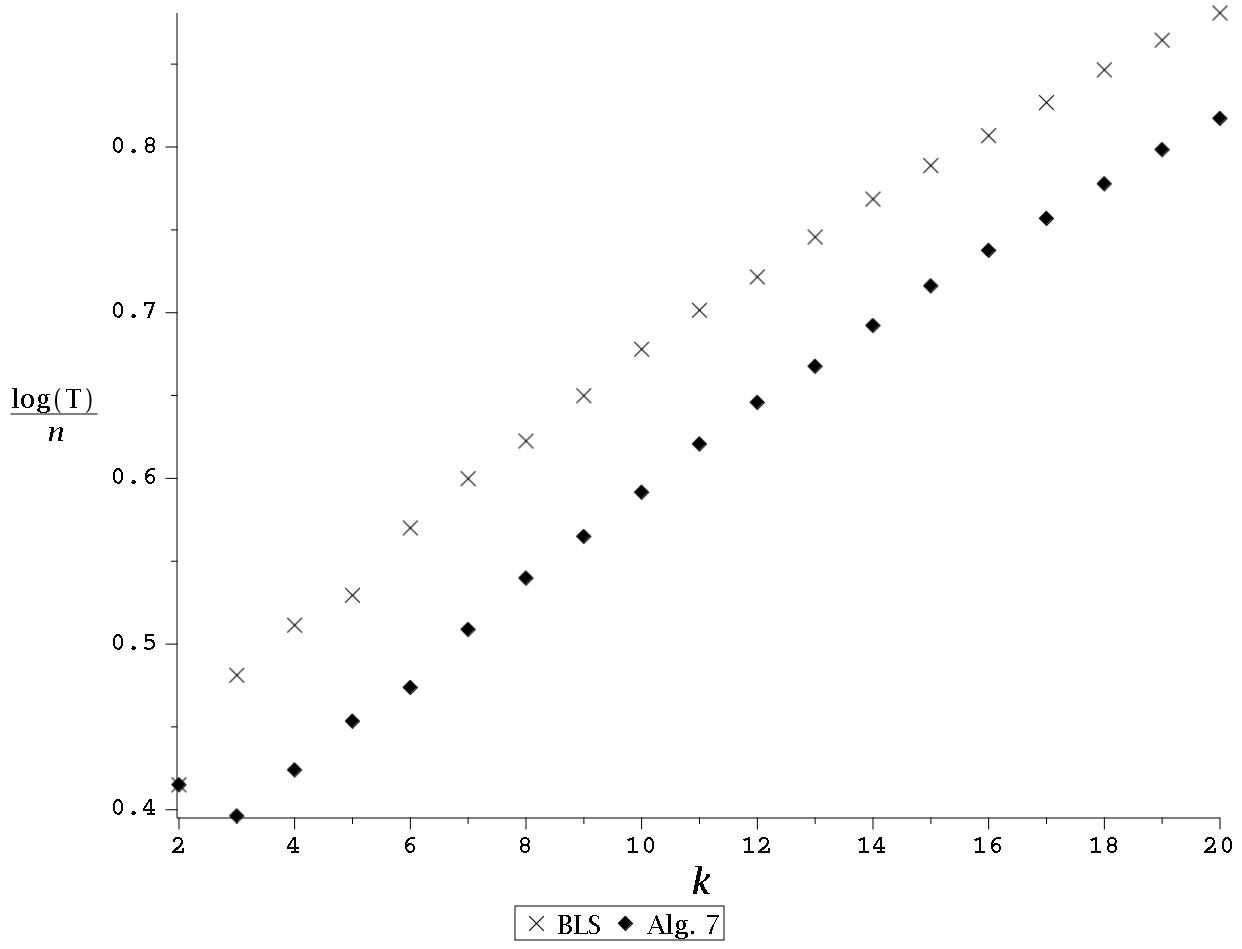
\includegraphics[scale=0.2]{kListRunTimesCompare}
	\hspace{4ex}
	\caption[Runtime exponents for $k$-List algorithms]{Running time exponents scaled by $1/n$ for the target length $t=1$. For $k=2$, both algorithms are the Nguyen-Vidick sieve \cite{NguVid08} with $\log(T)/n = 0.415$ (naive brute-force over two lists). For $k=3$, Algorithm \ref{alg:AlgConfig} achieves $\log(T)/n = 0.3962$, the BLS algorithm has $\log(T)/n = 0.4812$. \vspace{10ex}} \label{fig:RunTimes}
\end{SCfigure}

Our algorithm can be further improved by applying Locality-Sensitive Hashing techniques similar to \cite{SODA:BDGL16} to shorten the lists prior to filtering. Unfortunately, the gain is very modest: for $k=3, t=1$, we can get the running time down from $2^{0.3962n + \smallo(n)}$ to $2^{0.3717n + \smallo(n)}$. The details on this extension are presented in \cite{HK}.

We remark that it seems quite challenging to analyze the $k$-List algorithms for a \emph{non-fixed} $k$. Our approach heavily relies on the fact that $k$ is a fixed constant allowing to suppress all the pre-factors in both run-times and list sizes in the $\softO_k(\cdot)$ notation. Indeed, taking a closer look at the suppressed pre-factors, we immediately notice that they depend at least \emph{exponentially} on $k$ (see, for example, the expression for $W_{n,k}$ in Thm.~\ref{thm:WishartDist}). Being able to let $k \rightarrow \infty$ would, however, greatly contribute to our understanding of complexity of \SVP as it would enable us to compare sieving techniques with enumeration. 

Further, we do not know what is an optimal choice of $\eps$ given $k$ and $\normalabs{L}$. In Sect.~\ref{subsec:KListResults}, we present our experimental results for Alg.~\ref{alg:AlgConfig}, where we just try several $\eps$'s.

\subsection{Approximate Shortest Vector Problem} \label{subsec:ApproxSVP}

In this section we expound the connection between the approximate $k$-List problem in Euclidean norm (Def.~\ref{def:kListL2}) and the approximate Shortest Vector Problem, $\appSVP$, for a constant approximation factor $\gamma$. Recall the definition of the latter problem.

On input, we are given a full-rank lattice $\mathcal{L}(B)$ described by a matrix $B \in \R^{n \times n}$ (with polynomially-sized entries) and some constant $\gamma > 1$. The task is to output a non-zero lattice vector $\xvec \in \mathcal{L}(B)$ s.t.\ $ \| \xvec \| \leq \gamma \lambda_1 (B)$. $\xvec$ is a solution to the approximate shortest vector problem. Since the solution is not unique, we are fine with any vector that satisfies the length condition.

The family of so-called sieving (or \AKS) algorithms, described in the pioneering work of Ajtai, Kumar, and Sivakumar \cite{STOC:AjtKumSiv01}, offers the best known to-date heuristic algorithm for $\appSVP$. The fact that this algorithm achieves a single-exponential running time and memory complexity was already stated in the original paper \cite{STOC:AjtKumSiv01}, but a more precise analysis of the constant in the exponent has a long history. The result of Nguyen and Vidick in \cite{NguVid08}, stating the running time of order $2^{5.9n + \smallo(n)}$,  was later improved by Pujol and Stehl\'e to $2^{2.465n + \smallo(n)}$ running time and $2^{1.42n + \smallo(n)}$ space \cite{PujSte09}. Under an assumption on the distribution of lattice-vectors under sieving, we are able to \emph{heuristically} solve $\appSVP$ in $2^{0.415n + \smallo(n)}$ time and $2^{0.208n + \smallo(n)}$ space. Finally, the currently best known running time of  $2^{0.292n + \smallo(n)}$ in \cite{SODA:BDGL16} comes from a line of works based on the techniques from Locality-Sensitive Hashing. This is to be compared with the fastest \emph{provable} $\appSVP$ solver by Aggarwal et al.\ \cite{STOC:ADRS15}. Based on the so-called discrete Gaussian sampling, this algorithm achieves $2^{n + \smallo(n)}$-time and space complexity. 

Practically, however, sieving algorithms are less attractive than Kannan's enumeration with running time of order $2^{\bigO(n \log n)}$. This fact is attributed to exponential memory requirement of sieving (and also to the advances in pruning techniques for enumeration). Recently, Bai, Laarhoven, Stehl\'e aiming at reducing memory, presented a variant of sieving algorithm with space complexity of $2^{0.1887n+\smallo(n)}$ -- an exponential improvement over the previous $2^{0.208n + \smallo(n)}$-space sieving algorithm. Yet the gain comes at cost of increased running time: $2^{0.4812n + \smallo(n)}$ as opposed to $2^{0.415n +\smallo(n)}$ (for non-LSH sieving). To understand the BLS algorithm and how our improved $k$-List solver gives a faster sieving algorithm, we briefly explain how the \AKS algorithm works. 

\paragraph{The Nguyen-Vidick sieve.} Sieving algorithms have two flavours: the Nguyen-Vidick sieve \cite{NguVid08} and the Gauss sieve \cite{STOC:MicVou10}. Both make $\poly(n)$ number of calls to the approximate $2$-List solver. The Nguyen-Vidick sieve starts by sampling lattice-vectors $\xvec \in \Lat(B) \cap \Ball(\zerovec, 2^{\bigO(n)} \cdot \lambda_1(B))$. This can be done using, for example, Klein's sampling procedure \cite{SODA:Klein00} that outputs a lattice-vector of length not greater than $2^{\bigO(n)} \cdot \lambda_1(B)$.  In the $2$-List Nguyen-Vidick sieve, we sample many such lattice-vectors, put them in a list $L$, and search for \emph{pairs} $\xvec_1 \times \xvec_2 \in L \times L$ s.t. $\| \xvec_1 \pm \xvec_2 \| \leq (1-\eps) \max\{\| \xvec_1 \|, \| \xvec_2 \|\}$ for some small $\eps>0$. The sum is put into $\Lout$. The size of $L$ is chosen in a way to guarantee $\normalabs{L} \approx \normalabs{\Lout}$. The search for pairs is repeated over the list $\Lout$ once it is large enough. 

The size of $L$ determines the space complexity of the algorithm. A natural way to shorten the size of the input list $L$ is, instead of looking for pairs, look for triples, or, more general, $k$-tuples that form a short sum. Indeed, it easily follows from Cor.~\ref{cor:BalancedListSizes} that the larger $k$ is, the fewer vectors we should sample for the starting list  $L$ in order to expect $\normalabs{\Lout} = \normalabs{L}$. 

So the Nguyen-Vidick can be generalized to the search for $k$-tuples $\xvec_1, \ldots, \xvec_k \in L \times \ldots \times L$ s.t.\ $\| \xvec_1 + \ldots + \xvec_k \| \leq (1-\eps) \max_{1 \leq i \leq k} \{\| \xvec_i\|\}$. Now the sum $\xvec_1 + \ldots + \xvec_k$ is put into $\Lout$ and the search for $k$-tuples is repeated over $\Lout$. Note that since with each new iteration we obtain vectors that are shorter by a constant factor $(1-\eps)$, starting with $2^{\bigO(n)}$ approximation to the shortest vector (a property guaranteed by Klein's sampler applied to an \LLL-reduced basis), we need only $\poly(n)$ iterations to find the desired $\xvec \in \Lat(B)$.

Naturally, we can apply our Alg.~\ref{alg:AlgConfig} to $k$ copies of the list $L$ to implement the search for short sums. We do so by making a commonly used assumption: we assume the sampled lattice-vectors we put into the list lie uniformly on a spherical shell (on a very thin shell, essentially a sphere). The heuristic here is that it does not affect the behaviour of the algorithm. Intuitively, the discreteness of a lattice should not be `visible' to the algorithm (at least not in the search for the approximate shortest vector; as soon as we see the discreteness, the vectors are already short enough). We refer to \cite{NguVid08} for a more exhaustive discussion on this heuristic. 

The advantage in using our Alg.~\ref{alg:AlgConfig} instead of the BLS $k$-List search within an \appSVP algorithm is straightforward: the search for a `good' $k$-tuple is the routine that determines the complexity of the algorithm. So any improved algorithm for the approximate $k$-List problem immediately leads to a better \appSVP algorithm. 

\paragraph{Gauss sieve.} More interestingly, our improved $k$-List algorithm for $k \geq 3$ can as well be used within the Gauss sieve, which is known to perform faster in practice than the Nguyen-Vidick sieve. Let us briefly recall the Gauss sieve algorithm.

An iteration of the original 2-Gauss sieve as described in \cite{STOC:MicVou10}, searches for pairs $(\pvec, \vvec)$ s.t.\ $\| \pvec + \vvec \| < \max \{\| \pvec \|, \| \vvec \| \}$, where $\pvec \in \mathcal{L}(B)$ is \emph{fixed}, $\vvec \in L \subset \mathcal{L}(B)$, and $\pvec \neq \vvec$. Once such a pair is found and $\| \pvec \| > \| \vvec \|$, we reduce $\pvec$ by setting $\pvec'  \leftarrow \pvec + \vvec$ and proceed with the search over $(\pvec', \vvec)$, otherwise if $\| \pvec \| < \| \vvec \|$, we delete $\vvec \in L$ and store the sum $ \pvec + \vvec$ as $\pvec$-input point for the next iteration. Once no pair is found, we add $\pvec'$ to $L$. On the next iteration, the search is repeated with another $\pvec$ which is obtained either by reducing some previously deleted $\vvec \in L$, or by sampling from $\mathcal{L}(B)$. The idea is to keep only those vectors in $L$ that \emph{cannot} form a pair with a shorter sum. Bai, Laarhoven, and Stehl\'{e}  in \cite{BLS16}, generalize it to the $k$-Gauss sieve by keeping only those vectors in $L$ that do not form a shorter $k$-sum. In the language of configuration search, we look for configurations $(\pvec, \vvec_1, \ldots, \vvec_{k-1}) \in \pvec \times L \times \ldots \times L$ where the first point is fixed, so we apply our Alg.~\ref{alg:AlgConfig} on $k-1$ (identical) lists.

Pseudo-code for $3$-Gauss sieve is given in Alg.~\ref{alg:3GaussSieve} below. We assume the approximation $\gamma \lambda_1(B)$ is given as input. The main procedure (first lines 1-11) is exactly the same as in the original algorithm of Micciancio-Voulgaris. The difference is in the main subroutine $\Call{TripleReduce}$ that implements the approximate $3$-List search with the first vector in a triple being $\pvec$. The list $L$ is always kept sorted so that at the end of the procedure the shortest vector in the list is $L[1]$.
The algorithm can be easily generalized to the larger $k$, but we decided to present $k=3$ case as the most practically relevant. The experimental results on $3$-Gauss sieve are given in the next section.

\begin{algorithm}[t]
\caption{$3$-Gauss sieve}
\label{alg:3GaussSieve}
\textbf{Input:} $B \in \R^{n \times n}$ - an \LLL-reduced lattice basis, $\gamma \lambda_1(B)$ - the desired approximation factor, $\eps>0$ \\
\textbf{Output:} $\xvec \in \Lat(B)$ s.t.\ $\| \xvec \| \leq \gamma \lambda_1 (B)$

\begin{algorithmic}[1]
	\State $L \gets \{\}$ \Comment Sorted list of triple-reduced vectors
	\State $S \gets \{\}$ \Comment Stack of vectors
	\While{($L[1] > \gamma \lambda_1(B)$)}
		\If{$S$ is not empty}
			\State $\pvec \gets S.\text{pop()}$
		\Else
			\State $\pvec \gets \text{KleinSample}(B)$ \Comment Sample a vector from $\Lat(B)$
		\EndIf
		\State $\pvec' \gets $ \Call{TripleReduce}{$\protect \pvec, L, s$}
		\If{$\pvec' \neq \zerovec$}
			\State $L \gets L \union \{ \pvec'\}$
		\EndIf
	\EndWhile
	\State \Return $L[1]$
\end{algorithmic}

\vspace{10pt}

\begin{algorithmic}[1]
	\Function{TripleReduce}{$\protect \pvec, L, S$}
		\While{($\pvec$ cannot be reduced)} \Comment Try to reduced $\pvec$ first
			\State $L' \gets $ \Call{Filter}{$ \protect \pvec, L, \eps$}
			\ForAll{$\vvec_1, \vvec_2 \in L' \times L'$}
				\If{$\| \pvec \pm \vvec_1 \pm \vvec_2 \| < \| \pvec \|$}
					\State $\pvec \gets \vvec_1 \pm \vvec_2$ \Comment the sign should satisfy the If-condition
				\EndIf
			\EndFor
		\EndWhile
		\State $L' \gets $ \Call{Filter}{$ \protect \pvec, L$} \Comment with a new reduced $\pvec$
		\ForAll{$\vvec_1, \vvec_2 \in L' \times L'$}
			\If{$\| \pvec \pm \vvec_1 \pm \vvec_2 \| < \max \{ \| \vvec_1 \|, \| \vvec_2 \| \} $}
				\State $\max \{ \| \vvec_1 \|, \| \vvec_2 \| \} \gets \pvec \pm \vvec_1 \pm \vvec_2$
			\EndIf
		\EndFor
		\State \Return $\pvec$
	\EndFunction
\end{algorithmic}

\vspace{10pt}

\begin{algorithmic}[1]
	\Function{Filter}{$\protect \pvec, L, \eps$} \Comment Filter w.r.t.\@ balanced configuration $\Cbalt$
		\State $L' \gets \{ \}$
		\ForAll{$\vvec \in L$}
			\If{$\big| \frac{\langle \vvec, \pvec \rangle}{\|\vvec \| \|\pvec \|} \big| \geq \frac{1}{3} - \eps$}
				\State $L' \gets L' \union \{ \vvec \}$
			\EndIf
		\EndFor
		\State \Return $L'$
	\EndFunction
\end{algorithmic}

\end{algorithm}

\clearpage

\subsection{Experimental results} \label{subsec:KListResults}
We implement the $3$-Gauss sieve Algorithm~\ref{alg:3GaussSieve} in collaboration with S.\ Bai \cite{Bai16}. 
The implementation is based on the program developed by Bai, Laarhoven, and Stehl\'{e} in \cite{BLS16}. 
The experiments are run on the Ruhr University C3 cluster \cite{C3}. The results are presented in Table~\ref{table:kListExperiments}.

Lattice bases are generated by the \SVP challenge generator \cite{SVPChallenge}. It produces a lattice generated by the columns of the matrix
\begin{align*} B=
\begin{psmallmatrix}
	p & x_1 & \ldots & x_{n-1} \\
	0 & 1 & \ldots &  0  \\
	\vdots & \vdots & \ddots & \vdots \\
	0 & 0 & \ldots & 1 \\
\end{psmallmatrix},
\end{align*}
where $p$ is a large prime, and $x_i< p$ for all $i$. Lattices of this type are random in the sense of Goldstein and Mayer \cite{GoldMay06}.

For all the dimensions except $n=80$, the bases are preprocessed with \BKZ reduction of block-size~$20$. For $n=80$, the block-size is $30$. For our input lattices, we do not know their minimum $\lambda_1$. The algorithm terminates when it finds many linearly dependent triples $(\pvec, \vvec_1, \vvec_2)$. It means that at some point $\Call{TripleReduce}$ starts outputting $\zerovec$. We set a counter for such an event and terminate the algorithm once this counter goes over a pre-defined threshold. The intuition behind this idea is straightforward: at some point the list $L$ will contain very short basis-vectors and the remaining list-vectors will be their linear combinations. Trying to reduced the latter will ultimately produce the zero-vector. The same termination condition was already used in \cite{BLM15}, where the authors experimentally determine a threshold of such `zero-sum' triples.

Up to $n=64$, the experiments are repeated 5 times (i.e.\ on 5 random lattices), for the dimensions less than $80$, 3 times. For the running times and the list-sizes presented in the table below, the average is taken. For $n=80$, the experiment was performed once.  

Our tests confirm a noticeable speed-up of the 3-Gauss sieve when our Configuration Search Algorithm~\ref{alg:AlgConfig} is used. Moreover, as the analysis suggests (see Fig.~\ref{fig:RunTimes}), our algorithm outperforms the naive 2-Gauss sieve while using much less memory. 

Another interesting aspect of the algorithm is the list-sizes when compared with BLS. Despite the fact that asymptotically the size of the list $|L|$ is the same for our and for the BLS algorithms, in practice our algorithm requires a longer list (cf.\ the right numbers in each column). This is due to the fact that we filter out a larger fraction of solutions. Also notice that increasing $\eps$ -- the approximation to the target configuration -- we achieve an additional speed-up. This becomes obvious once we look at the $\Call{Filter}$ procedure: allowing for a smaller inner-product throws away less vectors, which in turn results in a shorter list $L$. For the range of dimensions we consider, the optimum is attained at $\eps=0.3$.

\renewcommand{\arraystretch}{1.9}
\begin{table}[t]
	\centering
	\resizebox{\textwidth}{!}{%
	\begin{tabular}{|c|c|c|c|c|c|c|} \hline
		 & \multirow{2}{*}{$2$-sieve} & \multirow{2}{*}{BLS $3$-sieve} & \multicolumn{4}{c|}{ Alg.~\ref{alg:3GaussSieve}, $3$-sieve} \\ \cline{4-7}
		& & & $\eps = 0.0$ & $\eps = 0.015$ & $\eps = 0.3$ & $\eps = 0.4$ \\ \hline
		$n$ & $T$, $\normalabs{L}$ & $T$, $\normalabs{L}$ & $T$, $\normalabs{L}$ & $T$, $\normalabs{L}$ & $T$, $\normalabs{L}$ & $T$, $\normalabs{L}$ \\ \hline
		60 & 1.38e3, 13257 & 1.02e4, 4936& 1.32e3, 7763& 1.26e3, 7386& 1.26e3, 6751 & \textbf{1.08e3, 6296} \\ \hline
		62 & 2.88e3, 19193 & 1.62e4, 6239 & 2.8e3, 10356 & 3.1e3, 9386 & \textbf{1.8e3, 8583} & 2.2e3, 8436 \\ \hline
		64 & 8.64e3, 24178 & 5.5e4, 8369 & 5.7e3, 13573& 3.6e3, 12369 & \textbf{3.36e3, 11142}& 4.0e4, 10934\\ \hline
		66 & 1.75e4, 31707 & 9.66e4, 10853 & 1.5e4, 17810 & 1.38e4, 16039 & \textbf{9.1e3, 14822}& 1.2e4, 14428 \\ \hline
		68 & 3.95e4, 43160 & 2.3e5, 14270 & 2.34e4, 24135 & 2.0e4, 21327 & \textbf{1.68e4, 19640}& 1.86e4, 18355 \\ \hline
		70 & 6.4e4, 58083 & 6.2e5, 19484 & 6.21e4, 32168 & 3.48e5, 26954 & \textbf{3.3e4, 25307} & 3.42e4, 24420 \\ \hline
		72 & 2.67e5, 77984 & 1.2e6, 25034& 7.6e4, 40671 & 7.2e4, 37091 & \textbf{6.16e4, 34063} & 6.35e4, 34032 \\ \hline
		74 & 3.45e5, 106654 & \textemdash& 2.28e5, 54198& 2.08e5, 47951& \textbf{2.02e5, 43661}& 2.03e5, 40882\\ \hline
		76 & 4.67e5, 142397 & \textemdash& 3.58e5, 71431& 2.92e5, 64620& \textbf{2.42e5, 56587} & 2.53e5, 54848 \\ \hline
		78 & 9.3e5, 188905 & \textemdash & \textemdash & \textemdash& \textbf{4.6e5, 74610} & 4.8e5, 70494 \\ \hline
		80 & \textemdash & \textemdash &\textemdash & \textemdash& \textbf{9.47e5, 98169} & 9.9e5, 98094\\ \hline
	\end{tabular}
	}	
	\caption[Experimental results for $k$-tuple Gauss sieve]{Experimental results for $k$-tuple Gauss sieve. The running times $T$ are given in seconds, $\abs{L}$ is the maximal size of the list $L$. $\eps$ is the approximation parameter for the subroutine $\Call{Filter}$ of Alg.~\ref{alg:3GaussSieve}. The best running-time per dimension is type-set bold.}
	\label{table:kListExperiments}
\end{table}